\documentclass[12pt, a4paper]{article}

% ============================================================
%  Packages
% ============================================================
\usepackage[utf8]{inputenc}
\usepackage[T1]{fontenc}
\usepackage[english]{babel}
\usepackage{amsmath, amssymb}
\usepackage{geometry}
\usepackage{booktabs}
\usepackage{array}
\usepackage{xcolor}
\usepackage{hyperref}
\usepackage{tikz}
\usetikzlibrary{arrows.meta, positioning, backgrounds, shapes.geometric, calc}

\geometry{margin=2.2cm}

% ---- Colores ----
\definecolor{depotcolor}{RGB}{220,50,50}      % rojo depósito (nodo 1)
\definecolor{deadnode}{RGB}{243,156,18}       % naranja: deadhanging nodes
\definecolor{servicenode}{RGB}{133,193,233}   % azul claro: solo servicio
\definecolor{bgedge}{RGB}{210,210,210}        % gris muy claro: fondo

% ---- Colores de ruta ----
\definecolor{routeA}{RGB}{52,152,219}   % azul fuerte
\definecolor{routeB}{RGB}{46,204,113}   % verde
\definecolor{routeC}{RGB}{155,89,182}   % morado
\definecolor{routeD}{RGB}{230,126,34}   % naranja oscuro
\definecolor{routeE}{RGB}{26,188,156}   % turquesa

\title{Deadhanging Nodes in the Initial Solution\\
       \large Worked Example on Instance \texttt{gdb1}}
\author{}
\date{}

% ============================================================
\begin{document}
\maketitle

% ------------------------------------------------------------
\section{Deadhanging Nodes en la Solución Inicial de GDB1}
% ------------------------------------------------------------

En el problema CARP, la representación interna de una solución almacena
únicamente las etiquetas de las tareas (\texttt{TR}$k$) que cada vehículo
debe servir, pero \emph{no} los nodos intermedios del grafo que el
vehículo recorre para desplazarse entre tareas consecutivas. Estos
desplazamientos vacíos se denominan \textbf{deadheading}, y su costo
se evalúa expandiendo cada par de tareas consecutivas mediante el
camino mínimo (Dijkstra) precomputado sobre el grafo $G$.

Definimos un \textbf{deadhanging node} como cualquier vértice
$w \in V$ que aparece como \emph{nodo intermedio} (es decir, ni inicial
ni final) en al menos uno de los caminos de deadheading que se
ejecutan al evaluar la solución. Aunque dichos nodos no se almacenan
explícitamente en la estructura de datos, son visitados físicamente
por el vehículo y forman parte del costo total de la ruta.

Para la instancia \texttt{gdb1} y su solución inicial,
los \textbf{deadhanging nodes} son
$\{2, 5, 6, 7, 8, 12\}$, mientras que los nodos
$\{3, 4, 9, 10, 11\}$ solo participan como extremos de tareas de
servicio. El depósito (nodo 1) es el extremo común de todas las rutas.

% ------------------------------------------------------------
\section*{Figura principal: Grafo GDB1 con rutas y deadheading}
% ------------------------------------------------------------

\begin{center}
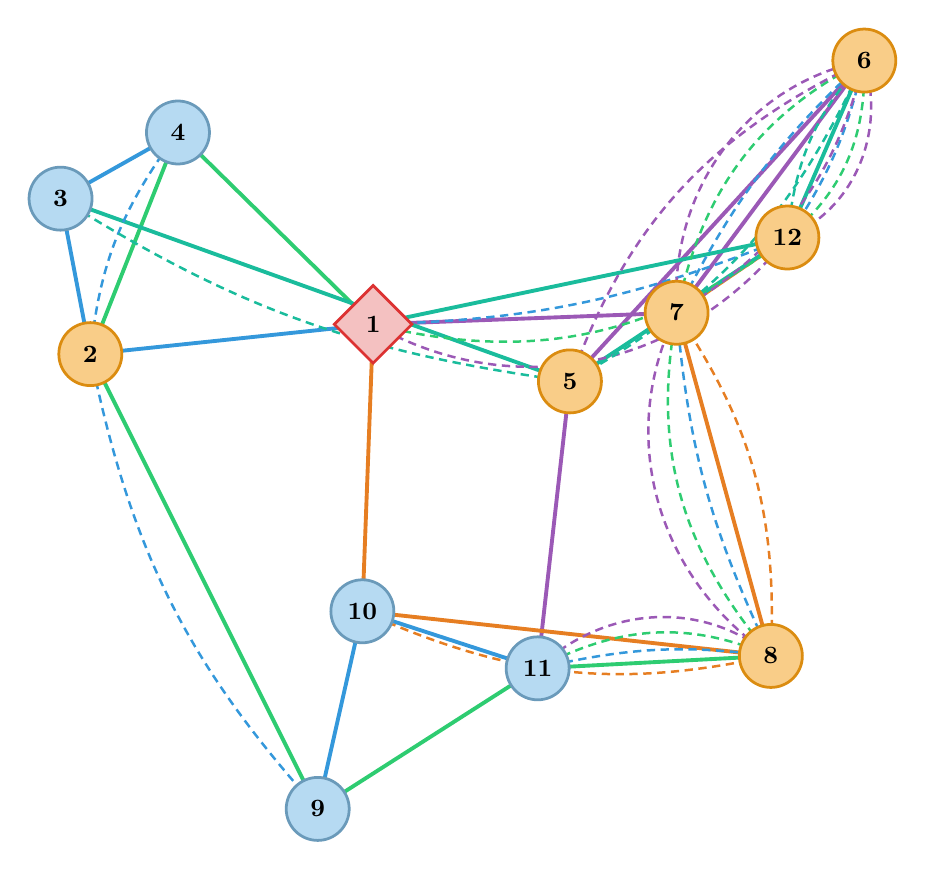
\begin{tikzpicture}[
    scale=1.05,
    every node/.style={font=\small\bfseries},
    depot/.style={diamond, draw=depotcolor, fill=depotcolor!30,
                  minimum size=10mm, line width=1.0pt,
                  inner sep=0pt},
    deadn/.style={circle, draw=deadnode!90!black, fill=deadnode!50,
                  minimum size=8mm, line width=1.0pt, inner sep=0pt},
    servn/.style={circle, draw=servicenode!80!black, fill=servicenode!60,
                  minimum size=8mm, line width=1.0pt, inner sep=0pt},
    bgedge/.style={draw=bgedge, line width=0.4pt},
    service/.style={-{Stealth[length=2.5mm]}, line width=1.4pt},
    deadhead/.style={-{Stealth[length=2.0mm]}, line width=0.9pt,
                     dash pattern=on 3pt off 2pt}
]

% ---- Coordenadas de los nodos (spring layout) ----
\coordinate (n1)  at (-1.12,  0.86);
\coordinate (n2)  at (-4.54,  0.50);
\coordinate (n3)  at (-4.90,  2.38);
\coordinate (n4)  at (-3.48,  3.18);
\coordinate (n5)  at ( 1.26,  0.17);
\coordinate (n6)  at ( 4.82,  4.05);
\coordinate (n7)  at ( 2.55,  1.00);
\coordinate (n8)  at ( 3.69, -3.15);
\coordinate (n9)  at (-1.79, -5.00);
\coordinate (n10) at (-1.25, -2.61);
\coordinate (n11) at ( 0.87, -3.30);
\coordinate (n12) at ( 3.89,  1.91);

% ============================================================
% Capa 1: TODOS los arcos del grafo en gris muy claro (fondo)
% ============================================================
\begin{scope}[on background layer]
  \draw[bgedge] (n1) -- (n2);
  \draw[bgedge] (n1) -- (n4);
  \draw[bgedge] (n1) -- (n7);
  \draw[bgedge] (n1) -- (n10);
  \draw[bgedge] (n1) -- (n12);
  \draw[bgedge] (n2) -- (n3);
  \draw[bgedge] (n2) -- (n4);
  \draw[bgedge] (n2) -- (n9);
  \draw[bgedge] (n3) -- (n4);
  \draw[bgedge] (n3) -- (n5);
  \draw[bgedge] (n5) -- (n6);
  \draw[bgedge] (n5) -- (n11);
  \draw[bgedge] (n5) -- (n12);
  \draw[bgedge] (n6) -- (n7);
  \draw[bgedge] (n6) -- (n12);
  \draw[bgedge] (n7) -- (n8);
  \draw[bgedge] (n7) -- (n12);
  \draw[bgedge] (n8) -- (n10);
  \draw[bgedge] (n8) -- (n11);
  \draw[bgedge] (n9) -- (n10);
  \draw[bgedge] (n9) -- (n11);
  \draw[bgedge] (n10) -- (n11);
\end{scope}

% ============================================================
% Capa 2: arcos de SERVICIO (flechas sólidas, color por ruta)
% ============================================================
% ---- Ruta 1 (azul fuerte): TR1(1,2) TR6(2,3) TR9(3,4) TR20(9,10) TR22(10,11) ----
\draw[service, color=routeA] (n1)  -- (n2);     % TR1
\draw[service, color=routeA] (n2)  -- (n3);     % TR6
\draw[service, color=routeA] (n3)  -- (n4);     % TR9
\draw[service, color=routeA] (n9)  -- (n10);    % TR20
\draw[service, color=routeA] (n10) -- (n11);    % TR22

% ---- Ruta 2 (verde): TR2(1,4) TR7(2,4) TR8(2,9) TR21(9,11) TR19(8,11) ----
\draw[service, color=routeB] (n1) -- (n4);      % TR2
\draw[service, color=routeB] (n2) -- (n4);      % TR7
\draw[service, color=routeB] (n2) -- (n9);      % TR8
\draw[service, color=routeB] (n9) -- (n11);     % TR21
\draw[service, color=routeB] (n8) -- (n11);     % TR19

% ---- Ruta 3 (morado): TR3(1,7) TR14(6,7) TR11(5,6) TR12(5,11) ----
\draw[service, color=routeC] (n1) -- (n7);      % TR3
\draw[service, color=routeC] (n6) -- (n7);      % TR14
\draw[service, color=routeC] (n5) -- (n6);      % TR11
\draw[service, color=routeC] (n5) -- (n11);     % TR12

% ---- Ruta 4 (naranja oscuro): TR4(1,10) TR18(8,10) TR16(7,8) TR17(7,12) ----
\draw[service, color=routeD] (n1)  -- (n10);    % TR4
\draw[service, color=routeD] (n8)  -- (n10);    % TR18
\draw[service, color=routeD] (n7)  -- (n8);     % TR16
\draw[service, color=routeD] (n7)  -- (n12);    % TR17

% ---- Ruta 5 (turquesa): TR5(1,12) TR13(5,12) TR10(3,5) TR15(6,12) ----
\draw[service, color=routeE] (n1)  -- (n12);    % TR5
\draw[service, color=routeE] (n5)  -- (n12);    % TR13
\draw[service, color=routeE] (n3)  -- (n5);     % TR10
\draw[service, color=routeE] (n6)  -- (n12);    % TR15

% ============================================================
% Capa 3: DEADHEADING con nodos intermedios (curvas, punteadas)
% Solo trazamos los DH que tienen al menos un nodo intermedio,
% ya que son los que generan deadhanging nodes.
% Usamos bend distintos para evitar solapamientos.
% ============================================================

% ---- Ruta 1: DH 4 -> 2 -> 9 (intermedio: 2) ----
\draw[deadhead, color=routeA] (n4) to[bend right=15] (n2);
\draw[deadhead, color=routeA] (n2) to[bend right=15] (n9);

% ---- Ruta 1: DH retorno 11 -> 8 -> 7 -> 6 -> 12 -> 1 (intermedios: 8,7,6,12) ----
\draw[deadhead, color=routeA] (n11) to[bend left=10] (n8);
\draw[deadhead, color=routeA] (n8)  to[bend left=10] (n7);
\draw[deadhead, color=routeA] (n7)  to[bend left=10] (n6);
\draw[deadhead, color=routeA] (n6)  to[bend left=10] (n12);
\draw[deadhead, color=routeA] (n12) to[bend left=10] (n1);

% ---- Ruta 2: DH retorno 11 -> 8 -> 7 -> 6 -> 12 -> 1 (intermedios: 8,7,6,12) ----
\draw[deadhead, color=routeB] (n11) to[bend left=25] (n8);
\draw[deadhead, color=routeB] (n8)  to[bend left=25] (n7);
\draw[deadhead, color=routeB] (n7)  to[bend left=25] (n6);
\draw[deadhead, color=routeB] (n6)  to[bend left=25] (n12);
\draw[deadhead, color=routeB] (n12) to[bend left=25] (n1);

% ---- Ruta 3: DH 7 -> 6 -> 5 (intermedio: 6) ----
\draw[deadhead, color=routeC] (n7) to[bend right=22] (n6);
\draw[deadhead, color=routeC] (n6) to[bend right=22] (n5);

% ---- Ruta 3: DH retorno 11 -> 8 -> 7 -> 6 -> 12 -> 1 (intermedios: 8,7,6,12) ----
\draw[deadhead, color=routeC] (n11) to[bend left=40] (n8);
\draw[deadhead, color=routeC] (n8)  to[bend left=40] (n7);
\draw[deadhead, color=routeC] (n7)  to[bend left=40] (n6);
\draw[deadhead, color=routeC] (n6)  to[bend left=40] (n12);
\draw[deadhead, color=routeC] (n12) to[bend left=40] (n1);

% ---- Ruta 4: DH 10 -> 8 -> 7 (intermedio: 8) ----
\draw[deadhead, color=routeD] (n10) to[bend right=18] (n8);
\draw[deadhead, color=routeD] (n8)  to[bend right=18] (n7);

% ---- Ruta 5: DH 12 -> 6 -> 5 (intermedio: 6) ----
\draw[deadhead, color=routeE] (n12) to[bend left=18] (n6);
\draw[deadhead, color=routeE] (n6)  to[bend left=18] (n5);

% ---- Ruta 5: DH 12 -> 6 -> 5 -> 3 (intermedios: 6,5) ----
% se omiten los dos primeros tramos (ya dibujados arriba con misma
% curvatura). Solo agregamos el tramo final 5->3 con leve curvatura
% distinta para diferenciarlo:
\draw[deadhead, color=routeE] (n5) to[bend left=12] (n3);

% ============================================================
% Capa 4: NODOS (encima de todas las aristas)
% ============================================================
\node[depot]  (N1)  at (n1)  {1};
\node[deadn]  (N2)  at (n2)  {2};
\node[servn]  (N3)  at (n3)  {3};
\node[servn]  (N4)  at (n4)  {4};
\node[deadn]  (N5)  at (n5)  {5};
\node[deadn]  (N6)  at (n6)  {6};
\node[deadn]  (N7)  at (n7)  {7};
\node[deadn]  (N8)  at (n8)  {8};
\node[servn]  (N9)  at (n9)  {9};
\node[servn]  (N10) at (n10) {10};
\node[servn]  (N11) at (n11) {11};
\node[deadn]  (N12) at (n12) {12};

\end{tikzpicture}
\end{center}

% ------------------------------------------------------------
\subsection*{Leyenda}
% ------------------------------------------------------------

\begin{center}
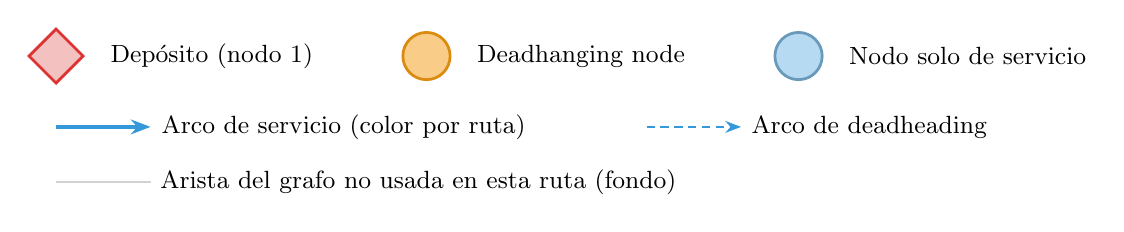
\begin{tikzpicture}[
    every node/.style={font=\small},
    depot/.style={diamond, draw=depotcolor, fill=depotcolor!30,
                  minimum size=7mm, line width=1pt, inner sep=0pt},
    deadn/.style={circle, draw=deadnode!90!black, fill=deadnode!50,
                  minimum size=6mm, line width=1pt, inner sep=0pt},
    servn/.style={circle, draw=servicenode!80!black, fill=servicenode!60,
                  minimum size=6mm, line width=1pt, inner sep=0pt}
]
% --- Fila 1: tipos de nodo ---
\node[depot] (l1) at (0,0) {};
\node[right=2mm of l1] (t1) {Depósito (nodo 1)};

\node[deadn, right=10mm of t1] (l2) {};
\node[right=2mm of l2] (t2) {Deadhanging node};

\node[servn, right=10mm of t2] (l3) {};
\node[right=2mm of l3] (t3) {Nodo solo de servicio};

% --- Fila 2: tipos de arco ---
\draw[-{Stealth[length=2.5mm]}, line width=1.4pt, color=routeA]
    (0,-0.9) -- ++(1.2,0) node[right, black] {Arco de servicio (color por ruta)};

\draw[-{Stealth[length=2.0mm]}, line width=0.9pt,
      dash pattern=on 3pt off 2pt, color=routeA]
    (7.5,-0.9) -- ++(1.2,0) node[right, black] {Arco de deadheading};

% --- Fila 3: aristas de fondo ---
\draw[draw=bgedge, line width=0.4pt]
    (0,-1.6) -- ++(1.2,0) node[right, black]
    {Arista del grafo no usada en esta ruta (fondo)};
\end{tikzpicture}
\end{center}

% ------------------------------------------------------------
\subsection*{Tabla resumen: tareas y deadhanging nodes por ruta}
% ------------------------------------------------------------

\begin{center}
\renewcommand{\arraystretch}{1.35}
\begin{tabular}{c l l}
\toprule
\textbf{Ruta} & \textbf{Tareas (secuencia)} &
\textbf{Deadhanging nodes} \\
\midrule
$r_1$ & \texttt{TR1 $\to$ TR6 $\to$ TR9 $\to$ TR20 $\to$ TR22}
      & $\{2,\; 6,\; 7,\; 8,\; 12\}$ \\
$r_2$ & \texttt{TR2 $\to$ TR7 $\to$ TR8 $\to$ TR21 $\to$ TR19}
      & $\{6,\; 7,\; 8,\; 12\}$ \\
$r_3$ & \texttt{TR3 $\to$ TR14 $\to$ TR11 $\to$ TR12}
      & $\{6,\; 7,\; 8,\; 12\}$ \\
$r_4$ & \texttt{TR4 $\to$ TR18 $\to$ TR16 $\to$ TR17}
      & $\{8\}$ \\
$r_5$ & \texttt{TR5 $\to$ TR13 $\to$ TR10 $\to$ TR15}
      & $\{5,\; 6\}$ \\
\midrule
\multicolumn{2}{r}{\textbf{Unión (deadhanging nodes globales)}}
      & $\{2,\; 5,\; 6,\; 7,\; 8,\; 12\}$ \\
\bottomrule
\end{tabular}
\end{center}

% ------------------------------------------------------------
\section{Descripción por Ruta}
% ------------------------------------------------------------

A continuación se listan los caminos de deadheading (con sus nodos
intermedios) que se ejecutan dentro de cada ruta al expandir la
solución inicial. El símbolo \textbf{negrita} resalta los nodos
\emph{intermedios} (deadhanging nodes), mientras que los nodos
extremos son siempre extremos de tareas de servicio.

\paragraph{Ruta 1 \textcolor{routeA}{$\blacksquare$}\;:}
$\texttt{D} \to \texttt{TR1}(1,2) \to \texttt{TR6}(2,3) \to
        \texttt{TR9}(3,4) \to \texttt{TR20}(9,10) \to
        \texttt{TR22}(10,11) \to \texttt{D}$
\begin{itemize}
  \item Deadhead $4 \to 9$: camino $[4,\;\mathbf{2},\;9]$, costo $= 11$
        \quad(intermedio: \textbf{2})
  \item Retorno $11 \to 1$: camino
        $[11,\;\mathbf{8},\;\mathbf{7},\;\mathbf{6},\;\mathbf{12},\;1]$,
        costo $= 29$ \quad(intermedios: \textbf{8, 7, 6, 12})
\end{itemize}

\paragraph{Ruta 2 \textcolor{routeB}{$\blacksquare$}\;:}
$\texttt{D} \to \texttt{TR2}(1,4) \to \texttt{TR7}(2,4) \to
        \texttt{TR8}(2,9) \to \texttt{TR21}(9,11) \to
        \texttt{TR19}(8,11) \to \texttt{D}$
\begin{itemize}
  \item Deadhead $4 \to 2$: camino $[4,\;2]$, costo $= 9$ (directo)
  \item Deadhead $11 \to 8$: camino $[11,\;8]$, costo $= 10$ (directo)
  \item Retorno $11 \to 1$: camino
        $[11,\;\mathbf{8},\;\mathbf{7},\;\mathbf{6},\;\mathbf{12},\;1]$,
        costo $= 29$ \quad(intermedios: \textbf{8, 7, 6, 12})
\end{itemize}

\paragraph{Ruta 3 \textcolor{routeC}{$\blacksquare$}\;:}
$\texttt{D} \to \texttt{TR3}(1,7) \to \texttt{TR14}(6,7) \to
        \texttt{TR11}(5,6) \to \texttt{TR12}(5,11) \to \texttt{D}$
\begin{itemize}
  \item Deadhead $7 \to 6$: camino $[7,\;6]$, costo $= 4$ (directo)
  \item Deadhead $6 \to 5$: camino $[6,\;5]$, costo $= 7$ (directo)
  \item Retorno $11 \to 1$: camino
        $[11,\;\mathbf{8},\;\mathbf{7},\;\mathbf{6},\;\mathbf{12},\;1]$,
        costo $= 29$ \quad(intermedios: \textbf{8, 7, 6, 12})
\end{itemize}

\paragraph{Ruta 4 \textcolor{routeD}{$\blacksquare$}\;:}
$\texttt{D} \to \texttt{TR4}(1,10) \to \texttt{TR18}(8,10) \to
        \texttt{TR16}(7,8) \to \texttt{TR17}(7,12) \to \texttt{D}$
\begin{itemize}
  \item Deadhead $10 \to 8$: camino $[10,\;8]$, costo $= 3$ (directo)
  \item Deadhead $8 \to 7$: camino $[8,\;7]$, costo $= 8$ (directo)
  \item Retorno $12 \to 1$: camino $[12,\;1]$, costo $= 4$ (directo,
        \emph{no produce deadhanging node})
\end{itemize}

\paragraph{Ruta 5 \textcolor{routeE}{$\blacksquare$}\;:}
$\texttt{D} \to \texttt{TR5}(1,12) \to \texttt{TR13}(5,12) \to
        \texttt{TR10}(3,5) \to \texttt{TR15}(6,12) \to \texttt{D}$
\begin{itemize}
  \item Deadhead $12 \to 5$: camino $[12,\;\mathbf{6},\;5]$,
        costo $= 10$ \quad(intermedio: \textbf{6})
  \item Deadhead $5 \to 6$: camino $[5,\;6]$, costo $= 7$ (directo)
  \item Retorno $12 \to 1$: camino $[12,\;1]$, costo $= 4$ (directo)
\end{itemize}

\paragraph{Observación.}
El nodo $12$ es \textbf{deadhanging} aunque también es extremo
de varias tareas de servicio (\texttt{TR5}, \texttt{TR13},
\texttt{TR15}, \texttt{TR17}): la clasificación se basa exclusivamente
en si el nodo aparece como \emph{intermedio} en algún camino mínimo
de deadheading. El nodo $5$, similarmente, es extremo de tareas
(\texttt{TR10}--\texttt{TR13}) y a la vez deadhanging porque
participa como intermedio en el deadhead $12 \to 6 \to 5 \to 3$
de la ruta 5. En cambio, los nodos $\{3,4,9,10,11\}$ nunca son
intermedios en ningún deadhead de esta solución, por lo que se
clasifican como \emph{solo de servicio}.

\end{document}
